\chapter{\glsentrylong{HEVC} (H.265)}
\label{cha:HEVC}

\section{Basics}
\begin{itemize}
\item Lossy and \popup{lossless}{Although by a large margin, it is
    mainly used as a lossy video codec.} \cite{wikipedia_HEVC}.
\item Standarized by the \gls{MPEG} and the \gls{VCEG} in 2013.
\item Is another (like \gls{MPEG}) video compression standard based on
  block-oriented, motion-compensated coding.
\end{itemize}

\section{Algorithm}
\label{sec:HEVC_algo}
\begin{itemize}
\item Similar to a \gls{AVC} codec (see Section~\ref{sec:MPEG-4_AVC_algo}),
  but \gls{HEVC}:
\begin{enumerate}
\item Larger MB (\gls{CTU}) sizes (up to $64\times 64$).
\item $32\times 32$ \gls{DCT}.
\item 1/8 pel motion compensation accuracy.
\item Larger prediction neighborhoods.
\item 35 intra prediction modes (directions).
\item Improved context modeling in \gls{CABAC}.
\item Improved motion vectors entropy coding.
\item Better deblocking filters.
\end{enumerate}
\end{itemize}

\section{Compression gain}

\begin{figure}[H]
  \vspace{+2ex}
  \centering
  \href{https://www.epiphan.com/blog/h264-vs-h265/}{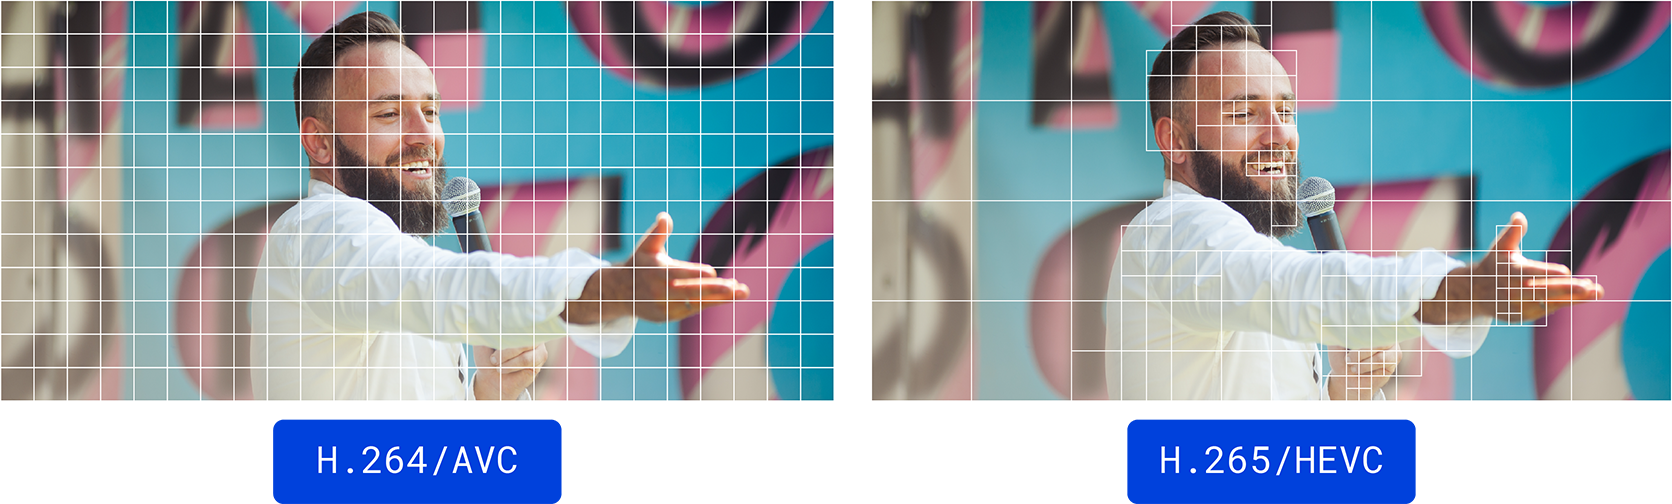
\includegraphics[width=\textwidth]{AVC-vs-HEVC}}
  \caption{\gls{HEVC} VS H.264/\gls{AVC}.}
  \label{fig:HEVC_vs_AVC}
\end{figure}

\begin{center}
\end{center}
